\documentclass[12pt]{article}
% Load packages
\usepackage{url}  % Formatting web addresses
\usepackage{ifthen}  % Conditional
\usepackage{multicol}   %Columns
\usepackage[utf8]{inputenc} %unicode support
\usepackage{amsmath}
\usepackage{amssymb}
\usepackage{epsfig}
\usepackage{epstopdf}
\usepackage{graphicx}
\usepackage[margin=0.1pt,font=footnotesize,labelfont=bf]{caption}
\usepackage{setspace}
%\usepackage{longtable}
\usepackage{colortbl}
%\usepackage{palatino,lettrine}
%\usepackage{times}
%\usepackage[applemac]{inputenc} %applemac support if unicode package fails
%\usepackage[latin1]{inputenc} %UNIX support if unicode package fails
\usepackage[wide]{sidecap}
%\usepackage[authoryear,round,comma,sort&compress]{natbib}
\usepackage[round,sort,comma,numbers,sort&compress]{natbib}
%\usepackage[authoryear,round]{natbib}
\usepackage{supertabular}
\usepackage{simplemargins}
\usepackage{fullpage}
\usepackage{comment}
\usepackage{lineno}
%\usepackage{chicago}
\usepackage{textcomp}
\usepackage{multirow}
\usepackage{amsmath}
\usepackage[linesnumbered,lined,boxed,commentsnumbered]{algorithm2e}
\DeclareMathOperator*{\argmin}{\arg\!\min}

\usepackage{algorithm2e}
\usepackage{algpseudocode}
%\usepackage[space]{cite}
\urlstyle{rm}

%\textwidth = 6.50 in
%\textheight = 9.5 in
%\oddsidemargin =  0.0 in
%\evensidemargin = 0.0 in
%\topmargin = -0.50 in
%\headheight = 0.0 in
%\headsep = 0.25 in
%\parskip = 0.15in
%\linespread{1.75}
\doublespace

%\bibliographystyle{chicago}
\bibliographystyle{plos2009}

\makeatletter
\renewcommand\subsection{\@startsection
	{subsection}{2}{0mm}
	{-0.05in}
	{-0.5\baselineskip}
	{\normalfont\normalsize\bfseries}}
\renewcommand\subsubsection{\@startsection
	{subsubsection}{2}{0mm}
	{-0.05in}
	{-0.5\baselineskip}
	{\normalfont\normalsize\itshape}}
\renewcommand\section{\@startsection
	{subsection}{2}{0mm}
	{-0.2in}
	{0.05\baselineskip}
	{\normalfont\large\bfseries}}
\renewcommand\paragraph{\@startsection
	{paragraph}{2}{0mm}
	{-0.05in}
	{-0.5\baselineskip}
	{\normalfont\normalsize\itshape}}
\makeatother

%Review style settings
%\newenvironment{bmcformat}{\begin{raggedright}\baselineskip20pt\sloppy\setboolean{publ}{false}}{\end{raggedright}\baselineskip20pt\sloppy}

%Publication style settings

% Single space'd bib -
\setlength\bibsep{0pt}

\renewcommand{\rmdefault}{phv}\renewcommand{\sfdefault}{phv}
\newcommand{\norm}[1]{\left\lVert#1\right\rVert}

% Change the number format in the ref list -
\renewcommand{\bibnumfmt}[1]{#1.}

% Change Figure to Fig.
\renewcommand{\figurename}{Fig.}


% Begin ...
\begin{document}
\begin{titlepage}
{\par\centering\textbf{\Large {An Effective Model of the Retinoic Acid Induced HL-60 Differentiation Program}}}
\vspace{0.05in}
{\par \centering \large{Ryan Tasseff, Holly A. Jensen, Wei Dai, Rodica P. Bunaciu$^{\dag}$, Johanna Congleton$^{\dag}$, Andrew Yen$^{\dag}$, and Jeffrey D. Varner$^{*}$}}
\vspace{0.10in}
{\par \centering {Robert Frederick Smith School of Chemical and Biomolecular Engineering} and {$^{\dag}$Department of Biomedical Sciences, {Cornell University, Ithaca NY 14853}}}
\vspace{0.1in}
{\par \centering \textbf{Running Title:}~Effective modeling of HL-60 differentiation}
\vspace{0.1in}
{\par \centering \textbf{To be submitted:}~\emph{Frontiers~in~Systems~Biology}}
\vspace{0.5in}
{\par \centering $^{*}$Corresponding author:}
{\par \centering Jeffrey D. Varner,}
{\par \centering Professor, Robert Frederick Smith School of Chemical and Biomolecular Engineering,}
{\par \centering 244 Olin Hall, Cornell University, Ithaca NY, 14853}
{\par \centering Email: jdv27@cornell.edu}
{\par \centering Phone: (607) 255 - 4258}
{\par \centering Fax: (607) 255 - 9166}
\end{titlepage}
\date{}
\thispagestyle{empty}
\pagebreak

\section*{Abstract}
In this study, we present an effective model All-Trans Retinoic Acid (ATRA)-induced differentiation of HL-60 cells.
The model describes a key architectural feature of ATRA-induced differentiation,
positive feedback between an ATRA-inducible signalsome complex involving many proteins including Vav1, a guanine nucleotide exchange factor,
and the activation of the mitogen activated protein kinase (MAPK) cascade.
The model, which was developed by integrating logical rules with kinetic modeling, was significantly smaller than previous models.
However, despite its simplicity, it captured key features of ATRA induced differentiation of HL-60 cells.
We identified an ensemble of effective model parameters using measurements taken from ATRA-induced HL-60 cells.
Using these parameters, model analysis predicted that MAPK activation was bistable as a function of ATRA exposure.
Conformational experiments supported ATRA-induced bistability.
These findings, combined with other literature evidence, suggest that positive feedback is central to a diversity of cell fate programs.

\clearpage

\setcounter{page}{1}

\linenumbers

\section*{Introduction}
Understanding the architecture of differentiation programs is an important therapeutic challenge.
Differentiation induction chemotherapy (DIC), using agents such as the vitamin A derivative all-trans retinoic acid (ATRA),
is a promising approach for the treatment of many cancers \cite{Bushue:2010aa,Tang:2011aa,Cheung:2012aa}.
For example, ATRA treatment induces remission in 80–90\% of promyelocytic leukemia (APL) PML-RAR$\alpha$-positive patients \cite{Nilsson:1984aa}, thereby transforming a fatal diagnosis into a manageable disease.
However, remission is sometimes not durable and relapsed cases exhibit emergent ATRA resistance \cite{Warrell:1993aa,Freemantle:2003aa}.
To understand the basis of this resistance, we must first understand the ATRA-induced differentiation program.
Toward this challenge, lessons learned in model systems, such as the lineage-uncommitted human myeloblastic cell line HL-60, could inform our analysis of the more
complex differentiation programs occurring in patients. Patient derived HL-60 leukemia cells have been a durable experimental model since the 1970’s to study differentiation \cite{Breitman1980}.
HL-60 undergoes cell cycle arrest and either myeloid or monocytic differentiation following stimulation; ATRA induces G1/G0-arrest and myeloid differentiation in HL-60 cells,
while 1,25-dihydroxy vitamin D3 (D3) induces arrest and monocytic differentiation.
Commitment to cell cycle arrest and differentiation requires approximately 48 hr of treatment,
during which HL-60 cells undergo two division cycles.

Sustained mitogen-activated protein kinase (MAPK) activation is a defining feature of ATRA-induced HL-60 differentiation.
ATRA drives sustained MEK-dependent activation of the Raf/MEK/ERK pathway, leading to arrest and differentiation \cite{Yen1998}.
MEK inhibition results in the loss of ERK and Raf phosphorylation, and the failure to arrest and differentiate \cite{Hong2001}.
ATRA (and its metabolites) are ligands for the hormone activated nuclear transcription factors retinoic acid receptor (RAR) and retinoid X receptor (RXR) \cite{Mangelsdorf1990}.
RAR/RXR activation is necessary for ATRA-induced Raf phosphorylation  \cite{Hong2001},
and the formation of an ATRA-inducible signalsome complex at the membrane which drives MAPK activation through a yet to be identified kinase activity.
While the makeup of the signalsome complex is not yet known,
we do know that it is composed of Src family kinases Fgr and Lyn, PI3K, c-Cbl, Slp76, and KSR, as well as IRF-1 transcription factors \cite{Congleton:2012fk,Shen:2011aa,Shen2009,Yen2006,Marchisio:1998aa}.
Signalsome formation and activity is driven by ATRA-induced expression of CD38 and the putative heterotrimeric Gq protein-coupled receptor BLR1 \cite{Congleton2011,WANG2004}.
BLR1, identified as an early ATRA (or D3)-inducible gene using differential display \cite{YEN1990},
is necessary for MAPK activation and differentiation \cite{WANG2004}, and is also involved with signalsome activity.
Studies of the BLR1 promoter identified a 5' 17bp GT box approximately 1 kb upstream of the transcriptional start that conferred ATRA responsiveness \cite{WANG2004}.
Members of the BLR1 transcriptional activator complex, e.g. NFATc3 and CREB,
are phosphorylated by ERK, JNK or p38 MAPK family members suggesting positive feedback between the signalsome and MAPK activation \cite{Yang2002}.
BLR1 overexpression enhanced Raf phosphorylation and accelerated terminal differentiation, while Raf inhibition reduced BLR1 expression and differentiation \cite{Wang2008}.
BLR1 knock-out cells failed to activate Raf or differentiate in the presence of ATRA \cite{Wang2008}.
Interestingly, both the knockdown or inhibition of Raf, also reduced BLR1 expression and functional differentiation \cite{Wang2008}.
Thus, the expression of signalsome components e.g., BLR1 was Raf dependent, while Raf activation depended upon the siganlsome.
A recent computational study of ATRA-induced differentiation in HL-60 cells suggested that the BLR1-MAPK positive feedback circuit was sufficient
to explain ATRA-induced sustained MAPK activation, and the expression of a limited number of functional differentiation markers \cite{Tasseff2011}.
Model analysis also suggested that Raf was the most distinct of the MAPK proteins.
However, this previous study developed and analyzed a complex model,
thus leaving open the critical question of what is the minimal positive feedback circuit required to drive ATRA-induced differentiation.

In this study, we explored this question using a minimal mathematical model of the key architectural feature of ATRA induced differentiation of HL-60 cells,
namely positive feedback between an ATRA-inducible signalsome complex and MAPK activation.
The ATRA responsive signalsome-MAPK circuit was then used to drive a downstream gene expression program which encoded for the expression of functional differentiation markers.
The effective model used a novel framework which integrated logical rules with kinetic modeling to describe gene expression and protein regulation,
while largely relying upon biophysical parameters from the literature.
This formulation significantly reduced the size and complexity of the model compared to the previous study of Tasseff et al., while increasing the breadth of the biology described \cite{Tasseff2011}.
The effective model, despite its simplicity, captured key features of ATRA induced differentiation of HL-60 cells.
Model analysis predicted the bistability of MAPK activation as a function of ATRA exposure; conformational experiments supported ATRA-induced bistability.
Model simulations were also consistent with measurements of the influence of MAPK inhibitors, and the failure of BLR1 knockout cells to differentiate when exposed to ATRA.
Lastly, we showed by through immunoprecipitation studies, that the guanine nucleotide exchange factor Vav1 is potentially a new ATRA-inducible member of the siganlsome complex.
Taken together, these findings when combined with other literature evidence,
suggested that positive feedback architectures are central to differentiation programs generally, and necessary for ATRA-induced differentiation.

% These findings, combined with other literature evidence, suggests that positive feedback architectures are central to
% many cell fate programs.
%Wang and Yen showed that ectopic expression of the constitutively active CR3 domain of Raf1 restored ATRA-induced G0 arrest and differentiation in BLR1 knock-out cells \cite{Wang2008}.
%However, ectopic expression of Raf1 CR3 alone, in the absence of ATRA, failed to induce arrest or differentiation in BLR1 knock-out cells.
%We identified an ensemble of effective model parameters using measurements taken from ATRA-induced HL-60 cells.
%Using these parameters,

\clearpage

\section*{Results}
We constructed an effective model of ATRA-induced HL-60 differentiation which described signaling and gene expression events following the addition of ATRA (Fig. \ref{fig:network}).
The model connectivity was developed from literature and the studies presented here (Table \ref{tbl:TF-network-connectivity}).
We decomposed the ATRA program into three modules;
a signal initiation module that sensed and transformed the ATRA signal into activated cRaf-pS621 and the ATRA-RXR/RAR (Trigger) signals (Fig. \ref{fig:network}A);
a signal integration module that controlled the expression of upstream transcription factors given cRaf-pS621 and activated Trigger signals (Fig. \ref{fig:network}B); and
a phenotype module which encoded the expression of functional differentiation markers from the ATRA-inducible transcription factors (Fig. \ref{fig:network}C).
Each component of these modules was described by a mRNA and protein balance equation.
Additionally, the signal initiation module also described the abundance of activated species e.g., Trigger and cRaf-pS621 whose values were derived from
unactivated Trigger and cRaf protein levels.
Lastly, because the population of HL-60 cells was dividing (at least before ATRA-induced cell cycle arrest), we also considered a dilution term in all balance equations.
The signal initiation module contained nine differential equations, while the signal integration and phenotype modules were collectively encoded by 54 differential equations.
Model parameters were taken literature (Table \ref{tbl:model-parameters}), or estimated from experimental data using heuristic optimization (see materials and methods).

The signal initiation module recapitulated sustained signalsome and MAPK activation following exposure to 1$\mu$M ATRA (Fig. \ref{fig:model-fitting}A-B).
An ensemble of effective model parameters was estimated by minimizing the difference between simulations and time-series measurements of BLR1 mRNA and
cRaf-pS621 following the addition of 1$\mu$M ATRA. We focused on the S621 phosphorylation site of cRaf since enhanced phosphorylation at this site is a defining
characteristic of sustained MAPK activation in HL-60. The effective model captured both ATRA-induced BLR1 expression (Fig. \ref{fig:model-fitting}A)
and sustained phosphorylation of cRaf-pS621 (Fig. \ref{fig:model-fitting}B) in a growing population of HL-60 cells.
Together, the reinforcing positive feedback between the signalsome and MAPK led to sustained activation over multiple cellular generations.
However, the effective model failed to capture the decline of BLR1 message after 48 hr of ATRA exposure.
This suggested that we captured the logic leading to the onset of differentiation, but failed to describe program shutdown.
Next, we tested the response of the signal initiation module to different ATRA dosages.

% Secondly, ATRA treatment alone increased both Raf phosphorylation at S621/S259 and Raf expression 24 hr post-treatment,
% while ATRA-induced phosphorylation of ERK was blocked by GW5074, consistent with the loss of Raf kinase activity (Fig. \ref{fig:ip-data}B).
% Lastly, both the phosphorylation and expression of Raf was inhibited by GW5074.
% This suggested a positive feedback between Raf kinase activity, Raf phosphorylation and ERK action on Raf transcription factors.

The signal initiation model was bistable with respect to ATRA induction (Fig. \ref{fig:model-fitting}C-D).
Phaseplane analysis predicted two stable steady-states when ATRA was present below a critical threshold (Fig. \ref{fig:model-fitting}C).
In the lower stable state, neither the signalsome nor cRaf-pS621 were present (thus, the differentiation program was deactivated).
However, at the high stable state, both the signalsome and cRaf-pS621 were present, allowing for sustained activation and differentiation.
Interestingly, when ATRA was above a critical threshold, only the activated state was accessible (Fig. \ref{fig:model-fitting}D).
To test these findings, we first identified the ATRA threshold. We exposed HL-60 cells to different ATRA concentrations for 72 hr (Fig. \ref{fig:model-fitting}E).
Morphological changes associated with differentiation were visible for ATRA $\geq$ 0.25 $\mu$M, suggesting the critical ATRA
threshold was near this concentration. Next, we conducted ATRA washout experiments to determine if activated cells remained activated in the absence of ATRA.
HL-60 cells locked into an activated state remained activated following ATRA withdraw (Fig. \ref{fig:model-predictions}).
This sustained activation resulted from reinforcing feedback between the signalsome and the MAPK pathway.
Thus, following activation, if we inhibited or removed elements from the signal initiation module we expected the siganlsome and MAPK signals to decay.
We simulated ATRA induced activation in the presence of kinase inhibitors, and without key circuit elements.
Consistent with experimental results using multiple MAPK inhibitors, ATRA activation in the presence of MAPK inhibitors lowered the steady-state value of signalsome (Fig. \ref{fig:model-predictions}A).
In the presence of BLR1, the signalsome and cRaf-pS621 signals were maintained following ATRA withdraw (Fig. \ref{fig:model-predictions}B, gray).
On the other hand, BLR1 deletion removed the ability of the circuit to maintain a sustained MAPK response following the withdraw of ATRA (Fig. \ref{fig:model-predictions}B, blue).
Lastly, washout experiments in which cells were exposed to 1$\mu$M ATRA for 24 hr, and then transferred to fresh media without ATRA,
confirmed the persistence of the self sustaining activated state for up to 144 hr (Fig. \ref{fig:model-predictions}C).
Thus, these experiments confirmed that reinforcing positive feedback likely drives the ATRA-induced differentiation program.
Next, we analyzed the ATRA-induced downstream gene expression program following signalsome and cRaf activation.

The signal integration and phenotype modules described ATRA-induced gene expression events in wild-type HL-60 cells (Fig. \ref{fig:model-grn-simulations}).
The signal initiation module produced two outputs, activated Trigger and cRaf-pS621 which drove the expression of ATRA-induced transcription factors,
which then in turn activated the phenotypic program. In particular, Trigger, which is a surrogate for the RAR$\alpha$/RXR transcriptional complex,
regulated the expression of the transcription factors CCATT/enhancer binding protein $\alpha$ (C/EBP$\alpha$), PU.1, and EGR1.
In turn, these transcription factors, in combination with cRaf-pS621, regulated the expression of downstream phenotypic markers such as CD38, CD11b or P47Phox.
We assembled the connectivity of the signal integration and phenotypic programs driven by Trigger and cRaf-pS621 from literature (Table \ref{tbl:TF-network-connectivity}).
We estimated the parameters which appeared in the control laws regulating these programs
from steady-state and dynamic measurements of transcription factor and phenotypic marker expression following the addition of ATRA [REFHERE].
However, the bulk of the remaining model parameters were taken from directly from literature \cite{Milo:2010aa} and were not estimated in this study (see materials and methods).
The model simulations captured the time dependent expression of CD38 and CD11b following the addition ATRA (Fig. \ref{fig:model-grn-simulations}A),
and the steady-state for signal integration and phenotypic markers (Fig. \ref{fig:model-grn-simulations}B).
Taken together, the signal integration and phenotypic simulations were consistent with measurements, thereby validating the assumed molecular connectivity.

% Vav1 is a member of an ATRA-inducible signalsome complex which propels sustained MAPK activation, arrest and differentiation (Fig. \ref{fig:network}B).
% We conducted immunoprecipitation studies and identified a limited number of ATRA-dependent and -independent Raf interaction partners.
% Of the 19 proteins sampled, Vav1, Src, CK2, Akt, and 14-3-3 precipitated with cRaf,
% suggesting a direct physical interaction was possible.
% However, only the associations between cRaf and Vav1 and Src were ATRA-inducible (Fig. \ref{fig:network}B).
% Others proteins e.g., CK2, Akt and 14-3-3, generally bound cRaf regardless of phosphorylation status or ATRA treatment.
% Treatment with the Raf kinase inhibitor GW5074 following ATRA exposure reduced the association of both Vav1 and Src with cRaf (Fig. \ref{fig:network}C),
% although the signal intensity for Src was weak.
% However, GW5074 did not influence the association of CK2 or 14-3-3 with cRaf,
% further demonstrating their independence from cRaf phosphorylation.
% Taken together, the immunoprecipitation and GW5074 results implicated Vav1 association to be correlated with cRaf activation following ATRA-treatment.

The composition of the siganlsome, and the kinase ultimately responsible for mediating ATRA-induced Raf activation is currently unknown.
To explore this question, we conducted immunoprecipitation and subsequent Western blotting to identify physical interactions between Raf and 19 putative interaction partners.
A panel of 19 possible Raf interaction partners (kinases, GTPases, scaffolding proteins etc)
was constructed based upon known signaling pathways.
We did not consider the most likely binding partner,
the small GTPase RAS, as previous studies have ruled it out in MAPK activation in HL-60 cells \cite{Wang2008,Katagiri1994}.
Total Raf was used as a bait protein for the immunoprecipitation studies.
Interrogation of the Raf interactome suggested Vav1 was involved with ATRA-induced initiation of MAPK activity (Fig. \ref{fig:ip-data}).
Western blot analysis using total Raf and pS621 Raf specific antibodies confirmed the
presence of the bait protein, total and phosphorylated forms, in the immunoprecipitate (Fig. \ref{fig:ip-data}A).
Of the 19 proteins sampled, Vav1, Src, CK2, Akt, and 14-3-3 precipitated with Raf, suggesting a direct physical interaction was possible.
However, only the associations between Raf and Vav1 and Raf and Src were ATRA-inducible (Fig. \ref{fig:ip-data}).
Furthermore, the Vav1 and Src associations were correlated with pS621 Raf abundance in the precipitate.
Others proteins e.g., CK2, Akt and 14-3-3, generally bound Raf regardless of phosphorylation status or ATRA treatment.
The remaining 14 proteins were expressed in whole cell lysate (Fig. \ref{fig:ip-data}B),
but were not detectable in the precipitate of Raf IP.
Treatment with the Raf kinase inhibitor GW5074 following ATRA exposure reduced the association of both Vav1 with Raf and Src with Raf (Fig. \ref{fig:ip-data}),
although the signal intensity for Src was notably weak.
However, GW5074 did not influence the association of CK2 or 14-3-3 with Raf, further demonstrating their independence from Raf phosphorylation.
Interestingly, the Raf-Akt interaction qualitatively increased following treatment with GW5074;
however, it remained unaffected by treatment with ATRA.
Src family kinases are known to be important in myeloid differentiation \cite{Miranda2007} and their role in HL-60 differentiation has been investigated elsewhere \cite{Congleton:2012fk}.
Given the existing work and variable reproducibility in the context of the Raf immunoprecipitate,
we did not investigate the role of Src further in this study.
Taken together, the immunoprecipitation and GW5074 results implicated Vav1 association to be correlated with Raf activation following ATRA-treatment.
Previous studies demonstrated that a Vav1-Slp76-Cbl-CD38 complex plays an important role in ATRA-induced MAPK activation and differentiation of HL-60 cells \cite{Shen2009}.
Here we did not observe direct interaction of Raf with Cbl or Slp76;
however, this complex could be involved upstream.

%For more details on GW5074 including dose response see Supplemental Materials including Fig. \ref{fig:ip-data}A.
Next, we considered the effect of the Raf kinase inhibitor GW5074 on functional markers of ATRA-induced growth arrest and differentiation.
Inhibition of Raf kinase activity modulated MAPK activation and differentiation markers following ATRA exposure (Fig. \ref{fig:ip-data}D-F).
ATRA treatment alone statistically significantly increased the G1/G0 percentage over the untreated control,
while GW5074 alone had a negligible effect on the cell cycle distribution (Fig. \ref{fig:ip-data}D).
Surprisingly, the combination of GW5074 and ATRA statistically significantly increased the G1/G0 population (82 $\pm$ 1\%)
compared with ATRA alone (61 $\pm$ 0.5\%).
Increased G1/G0 arrest following the combined treatment with GW5074 and ATRA was unexpected,
as the combination of ATRA and the MEK inhibitor (PD98059) has been shown previously to decrease ATRA-induced growth arrest \cite{Yen1998}.
However, growth arrest is not the sole indication of functional differentiation.
Expression of the cell surface marker CD11b has also been shown to coincide with HL-60 cells myeloid differentiation \cite{Hickstein1989}.
We measured CD11b expression, for the various treatment groups, using immuno-fluorescence flow cytometry 48 hr post-treatment.
As with G1/G0 arrest, ATRA alone increased CD11b expression over the untreated control,
while GW5074 further enhanced ATRA-induced CD11b expression (Fig. \ref{fig:ip-data}E).
GW5074 alone had no statistically significant effect on CD11b expression, compared with the untreated control.
Lastly, the inducible reactive oxygen species (ROS) response was used as a functional marker of differentiated neutrophils \cite{Congleton2011}.
We measured the ROS response induced by the phorbol ester 12-O-tetradecanoylphorbol-13-acetate (TPA) using flow cytometry.
Untreated cells showed no discernible TPA response,
with only 7.0 $\pm$ 3.0\% ROS induction (Fig. \ref{fig:ip-data}F).
Cells treated with ATRA had a significantly increased TPA response, 53 $\pm$ 7\% ROS induction 48 hr post-treatment.
Treatment with both ATRA and GW5074 statistically significantly reduced ROS induction (22 $\pm$ 0.6\%) compared to ATRA alone.
Interestingly, Western blot analysis did not detect a GW5074 effect on ATRA-induced expression of p47phox,
a required upstream component of the ROS response  (Fig. \ref{fig:ip-data}F, bottom).
Thus, the inhibitory effect of GW5074 on inducible ROS might occur downstream of p47phox expression.
However, the ROS producing complex is MAPK dependent,
therefore it is also possible that GW5074 inhibited ROS production by interfering
with MAPK activation (in which case the p47Phox marker might not accurately reflect phenotypic conversion and differentiation).

\clearpage

\section*{Discussion}
In this study, we presented an effective model of ATRA-inducible differentiation of HL-60 cells which
encoded positive feedback between the ATRA-inducible signalsome complex and the MAPK pathway.
Despite its simplicity, the model captured key features of the ATRA induced differentiation such as
sustained MAPK activation, and bistability with respect to ATRA exposure. We also reported a new ATRA-inducible component of the signalsome, Vav1.
Vav1 is a guanine nucleotide exchange factor for Rho family GTPases that activate pathways leading to actin cytoskeletal rearrangements and transcriptional alterations \cite{Hornstein:2004aa}.
The Vav1/Raf association correlated with Raf activity, was ATRA-inducible and decreased after treatment with GW5074.
The presence of Vav1 in Raf/Grb2 complexes has been shown to correlate with increased Raf activity in mast cells \cite{Song1996}.
Furthermore, studies on Vav1 knockout mice demonstrated that the loss of Vav1 resulted in deficiencies
of ERK signaling for both T-cells as well as neutrophils \cite{Costello1999,Graham2007}.
While its function in the signalsome is unclear, Vav1 has been shown to associate with a Cbl-Slp76-CD38 complex in an ATRA-dependent manner;
furthermore, transfection of HL-60 cells with Cbl mutants that fail to bind CD38, yet still bind Slp76 and Vav1, prevented
ATRA-induced MAPK activation \cite{Shen2009}. Thus, interaction of Cbl-Slp76-Vav1 and CD38 appears to be required for transmission of the ATRA signal by the
signalsome.

We conducted immunoprecipitation studies and identified a limited number of ATRA-dependent and -independent Raf interaction partners.
While we were unable to detect the association of Raf with common kinases and GTPases such as PKC, PKA, p38, Rac and Rho,
we did establish potential interactions between Raf and key partners such as Vav1, Src, Akt, CK2 and 14-3-3.
All of these partners are known to be associated with Raf activation or function.
Src is known to bind Raf through an SH2 domain, and this association has been shown to be dependent of the serine phosphorylation of Raf \cite{Cleghon1994}.
Thus, an ATRA inducible Src/Raf association may be a result of ATRA-induced Raf phosphorylation at S259 or S621.
We also identified an interaction between Raf and the Ser/Thr kinases Akt and CK2.
Akt can phosphorylate Raf at S259, as demonstrated by studies in a human breast cancer line \cite{Zimmermann1999}.
CK2 can also phosphorylate Raf, although the literature has traditionally focused on S338 and not S621 or S259\cite{Ritt2007}.
However, neither of these kinase interactions were ATRA-inducible, suggesting their association with Raf alone was not associated with ATRA-induced Raf phosphorylation.
The adapter protein 14-3-3 was also constitutively associated with Raf.
The interaction between Raf and 14-3-3 has been associated with both S621 and S259 phosphorylation and activity \cite{Hekman2004}.
Additionally, the association of Raf with 14-3-3 not only stabilized S621 phosphorylation,
but also reversed the S621 phosphorylation from inhibitory to activating \cite{Dhillon2009}.
Finally, we found that Vav1/Raf association correlated with Raf activity, was ATRA-inducible and decreased after treatment with GW5074.
The presence of Vav1 in Raf/Grb2 complexes has been shown to correlate with increased Raf activity in mast cells \cite{Song1996}.
Furthermore, studies on Vav1 knockout mice demonstrated that the loss of Vav1 resulted in deficiencies
of ERK signaling for both T-cells as well as neutrophils \cite{Costello1999,Graham2007}.
Interestingly, while an integrin ligand-induced ROS response was blocked in Vav1 knockout neutrophils, TPA was able to bypass the Vav1 requirement and stimulate both ERK phosphorylation
and ROS induction \cite{Graham2007}.
In this study, the TPA-induced ROS response was dependent upon Raf kinase activity, and was mitigated by the addition of GW5074.
It is possible that Vav1 is downstream of various integrin receptors but upstream of Raf in terms of inducible ROS responses.
Vav1 has also been shown to associate with a Cbl-Slp76-CD38 complex in an ATRA-dependent manner;
furthermore, transfection of HL-60 cells with Cbl mutants that fail to bind CD38, yet still bind Slp76 and Vav1, prevents
ATRA-induced MAPK activation \cite{Shen2009}.
The literature suggest a variety of possible receptor-signaling pathways, which involve Vav1, for MAPK activation; moreover,
given the ATRA-inducible association Vav1 may play a direct role in Raf activation.


We hypothesized that Vav1 is a member of an ATRA-inducible complex which propels sustained MAPK activation, arrest and differentiation.
Initially, ATRA-induced Vav1 expression drives increased association between Vav1 and Raf.
This increased interaction facilitates phosphorylation and activation of Raf by pre-bound Akt and/or CK2 at S621 or perhaps S259.
Constitutively bound 14-3-3 may also stabilize the S621 phosphorylation, modulate the activity and/or up-regulate autophosphorylation.
Activated Raf can then drive ERK activation, which in turn closes the positive feedback loop by activating Raf transcription factors,
e.g. Sp1 and/or STAT1 \cite{Kim2009,Milanini-Mongiat2002,Zhang2004,Li2006}.
We tested this working hypothesis using mathematical modeling.
The model recapitulated both ATRA time-course data as well as the GW5074 inhibitor effects.
This suggested the proposed Raf-Vav1 architecture was at least consistent with the experimental studies.
Further, analysis of the Raf-Vav1 model identified bistability in ppERK levels.
Thus, two possible MAPK activation branches were possible for experimentally testable ATRA values. The analysis also suggested the ATRA-induced Raf-Vav1 architecture could be locked into a
sustained signaling mode (high ppERK) even in the absence of a ATRA signal.
This locked-in property could give rise to an ATRA-induction memory.
We validated the treatment memory property predicted by the Raf-Vav1 circuit experimentally using ATRA-washout experiments.
ERK phosphorylation levels remained high for more then 96 hr after ATRA was removed.
Previous studies demonstrated that HL-60 cells possessed an inheritable memory of ATRA stimulus \cite{YEN1984}.
Although the active state was self-sustaining, the inactive state demonstrated considerable robustness to perturbation.
For example, we found that 50x overexpression of Raf was required to reliably lock MAPK into the activated state, while small perturbations had almost no effect on ppERK levels
over the entire ensemble.
CD38 expression correlated with the ppERK, suggesting its involvement in the signaling complex.
Our computational and experimental results showed that positive feedback,
through ERK-dependent Raf expression, could sustain MAPK signaling through many division cycles.
Such molecular mechanisms could underly aspects of cellular memory associated to consecutive ATRA treatments.

Several engineered, or naturally occurring systems involved in cell fate decisions incorporate positive feedback and bistability \cite{Ferrell:2002aa}.
One of the most well studied cell fate circuits is the Mos mitogen-activated protein kinase cascade in \textit{Xenopus} oocytes.
This cascade is activated when oocytes are induced by the steroid hormone progesterone \cite{Xiong:2003aa}.
The MEK-dependent activation of p42 MAPK stimulates the accumulation of the Mos oncoprotein, which in turn activates MEK, thereby closing the feedback loop.
This is similar to the differentiation circuit presented here; ATRA drives signalsome which activates MAPK, cell-cycle arrest, differentiation and signalsome.
Thus, while HL-60 and \textit{Xenopus} oocytes are vastly different biological models, they share similar cell fate decision architectures.
Other unrelated cell fate decisions such as programmed cell death have also been suggested to be bistable \cite{Bagci:2006aa}.
Still more biochemical networks important to human health, for example the human coagulation or complement cascades, also feature strong positive feedback elements \cite{Luan:2007aa}.
Thus, while positive feedback is sometimes not desirable in man made systems, it may be at the core of a diverse variety of
cell fate programs and other networks important to human health.

Model performance was impressive given its limited size. However, there were several issues to explore further.
First, there was likely missing connectivity in the effective differentiation circuit.
Decreasing BLR1 expression with simultaneously sustained cRaf-pS261 activation was not captured by the current network architecture.
This suggested that signalsome, once activated, had a long lifetime as decreased BLR1 expression did not impact cRaf-pS261 abundance.
We could model this by separating siganlsome formation into an inactive precursor pool that is transformed to a long-lived activated siganlsome by MAPK activation.
We should also explore adding additional downstream biological modules to this skeleton model, for example the upregulation of reactive oxygen markers such as p47Phox or
cell cycle arrest components to capture the switch from an actively proliferating population to a population in G0-arrest.
Next, the choice of max/min integration rules or the particular form of the transfer functions could also be explored.
Integration rules other than max/min could be used, such as the mean or the product, assuming the range of the transfer functions is always $f\in[0,1]$.
Alternative integration rules might have different properties which could influence model identification or performance.
For example, a mean integration rule would be differentiable, allowing derivative-based optimization approaches to be used.
The form of the transfer function could also be explored. We choose hill-like functions because of their
prominence in the systems and synthetic biology community. However, many other transfer functions are possible.

\clearpage

\section*{Materials and Methods}

\subsubsection*{Effective gene expression model equations.}
We decomposed the ATRA-induced differentiation program into three modules;
a signal initiation module that sensed and transformed the ATRA signal into activated cRaf-pS621 and the ATRA-RXR/RAR (activated Trigger) signals;
a signal integration module that controlled the expression of upstream transcription factors given cRaf-pS621 and activated Trigger signals; and
a phenotype module which encoded the expression of functional differentiation markers from the ATRA-inducible transcription factors.
The output of the signal initiation module was the input to the gene expression model.
For each gene $j=1,2,\dots,\mathcal{G}$, we modeled both the mRNA ($m_{j}$), protein ($p_{j}$) and signaling species abundance:
\begin{eqnarray}
	\frac{dm_{j}}{dt} &=& r_{T,j} - \left(\mu+\theta_{m,j}\right)m_{j}+\lambda_{j}\\
	\frac{dp_{j}}{dt} &=& r_{X,j} - \left(\mu+\theta_{p,j}\right)p_{j}\\\label{eqn-signaling-balances}
	\mathbf{g}\left(p_{1},\hdots,p_{\mathcal{G}},\kappa\right) &=& \mathbf{0}
\end{eqnarray}
The terms $r_{T,j}$ and $r_{X,j}$ denote the specific rates of transcription, and translation while
the terms $\theta_{m,j}$ and $\theta_{p,j}$ denote first-order degradation constants for mRNA and protein, respectively.
The specific transcription rate $r_{T,j}$ was modeled as the product of a kinetic term $\bar{r}_{T,j}$ and a control term $u_{j}$ which described how the
abundance of transcription factors, or other regulators influenced the expression of gene $j$.
The kinetic transcription term $\bar{r}_{T,j}$ was modeled as:
\begin{equation}
	\bar{r}_{T,j} = V^{max}_{T}\left(\frac{L_{T,o}}{L_{T,j}}\right)\left(\frac{G_{j}}{K_{T}+G_{j}}\right)
\end{equation}where the maximum gene expression rate $V^{max}_{T}$ was defined as the product of a characteristic transcription rate constant ($k_{T}$)
and the abundance of RNA polymerase ($R_{1}$), $V^{max}_{T} = k_{T}\left(R_{1}\right)$.
The $\left(L_{T,o}/L_{T,j}\right)$ term denotes the ratio of transcription read lengths; $L_{T,o}$ represents a characteristic gene length, while $L_{T,j}$ denotes the length of gene $j$.
Thus, the ratio $\left(L_{T,o}/L_{T,j}\right)$ is a gene specific correction to the characteristic transcription rate $V^{max}_{T}$.
The degradation rate constants were defined as $\theta_{m,j}$ and $\theta_{p,j}$ denote characteristic degradation constants for mRNA and protein, respectively.
Lastly, the $\lambda_{j}$ term denotes the constitutive rate of expression of gene $j$.

The gene expression control term $0\leq u_{j}\leq 1$ depended upon the combination of factors which influenced the expression of gene $j$.
If the expression of gene $j$ was influenced by $1,\dots,m$ factors, we modeled this relationship as
$u_{j}=\mathcal{I}_{j}\left(f_{1j}\left(\cdot\right),\hdots,f_{mj}\left(\cdot\right)\right)$
where $0\leq f_{ij}\left(\cdot\right)\leq 1$ denotes a regulatory transfer function quantifying the influence of factor $i$ on the expression of gene $j$,
and $\mathcal{I}_{j}\left(\cdot\right)$ denotes an integration rule which combines the individual regulatory inputs for gene $j$ into a single control term.
In this study, the integration rule governing gene expression was the weighted fraction of promoter configurations that resulted in gene expression \cite{Moon:2012ab}:
\begin{equation}
	{u}_{j} = \frac{W_{R_{1},j}+\displaystyle\sum_{n}W_{nj}f_{nj}}{1+W_{R_{1},j}+\displaystyle\sum_{d}W_{dj}f_{dj}}
\end{equation}
The numerator, the weighted sum (with weights $W_{nj}$) of promoter configurations leading to gene expression, was normalized by all possible promoter configurations.
The likelihood of each configuration was quantified by the transfer function $f_{nj}$ (which we modeled using hill like functions), while
the lead term in the numerator $W_{R_{1},j}$ denotes the weight of constitutive expression for gene $j$.
Given this formulation, the rate of constitutive expression was then given by:
\begin{equation}
	\lambda_{j} = \bar{r}_{T,j}\left(\frac{W_{R_{1},j}}{1+W_{R_{1},j}}\right)
\end{equation}
If a gene expression process had no modifying factors, $u_{j}=1$.
Lastly, the specific translation rate was modeled as:
\begin{equation}
	r_{X,j} = V^{max}_{X}\left(\frac{L_{X,o}}{L_{X,j}}\right)\left(\frac{m_{j}}{K_{X}+m_{j}}\right)
\end{equation}
where $V^{max}_{X}$ denotes a characteristic maximum translation rate estimated from literature, and $K_{X}$ denotes a translation saturation constant.
The characteristic maximum translation rate was defined as the product of a characteristic translation rate constant ($k_{X}$)
and the Ribosome abundance ($R_{2}$), $V^{max}_{X} = k_{X}\left(R_{2}\right)$. As was the case for transcription,
we corrected the characteristic translation rate by the ratio of the length of a characteristic transcription normalized by the length of transcript $j$.

\subsubsection*{Signaling model equations.}
The signal initiation, and integration modules required the level of cRaf-pS621 and ATRA-RXR/RAR (activated Trigger) as inputs.
However, our base model described only the abundance of inactive proteins e.g., cRaf or RXR/RAR but not the activated forms.
To address this issue, we estimated pseudo steady state approximations for the abundance of cRaf-pS621 and activated Trigger (shown generally as Eq \eqref{eqn-signaling-balances}).
The abundance of activated trigger ($x_{a,1}$) was estimated directly from the RXR/RAR abundance ($x_{u,1}$):
\begin{equation}
	x_{a,1} \sim x_{u,1}\left(\frac{\alpha\cdot{\mathrm{ATRA}}}{1+\alpha\cdot\mathrm{ATRA}}\right)
\end{equation}
where $\alpha$ denotes a gain parameter; $\alpha = 0.0$ if ATRA is less than a threshold, and $\alpha = 0.1$ if ATRA is greater than the differentiation threshold.
The abundance of cRaf-pS621 was estimated by making the pseudo steady state approximation on the cRaf-pS621 balance.
The abundance of an activated signaling species $i$ was given by:
\begin{equation}
	\frac{dx_{i}}{dt}  =  r_{+,i}\left(\mathbf{x},\mathbf{k}\right) - \left(\mu+k_{d,i}\right)x_{i}\qquad{i=1,\hdots,\mathcal{M}}\\
\end{equation}
The quantity $x_{i}$ denotes concentration of signaling species $i$, while $\mathcal{R}$ and $\mathcal{M}$ denote the number of signaling reactions and signaling species in the model,
respectively. The term $r_{+,i}\left(\mathbf{x},\mathbf{k}\right)$ denotes the rate of generation of activated species $i$,
while $\mu$ denotes the specific growth rate, and $k_{d,i}$ denotes the rate constant controlling the non-specific degradation of $x_{i}$.
We neglected deactivation reactions e.g., phosphatase activities.
We assumed that signaling processes were fast compared to gene expression; this allowed us to approximate the signaling balance as:
\begin{equation}
	x_{i}^{*} \simeq \frac{r_{+,i}\left(\mathbf{x},\mathbf{k}\right)}{\left(\mu+k_{d,i}\right)} \qquad{i=1,\hdots,\mathcal{M}}
\end{equation}
The generation rate was written as the product of a kinetic term ($\bar{r}_{+,i}$) and a control term ($v_{i}$).
The control terms $0\leq v_{j}\leq 1$ depended upon the combination of factors which influenced rate process $j$.
If rate $j$ was influenced by $1,\dots,m$ factors, we modeled this relationship as
$v_{j}=\mathcal{I}_{j}\left(f_{1j}\left(\cdot\right),\hdots,f_{mj}\left(\cdot\right)\right)$
where $0\leq f_{ij}\left(\cdot\right)\leq 1$ denotes a regulatory transfer function quantifying the influence of factor $i$ on rate $j$.
The function $\mathcal{I}_{j}\left(\cdot\right)$ is an integration rule which maps the output of regulatory transfer functions into a control
variable. In this study, we used $\mathcal{I}_{j}\in\left\{min,max\right\}$ and hill transfer functions \cite{pr3010138}.
If a process had no modifying factors, $v_{j}=1$.
The kinetic rate of cRaf-pS621 generation $\bar{r}_{+,cRaf}$ was modeled as:
\begin{equation}
	\bar{r}_{+,cRaf} = k_{+,cRaf}x_{s}\left(\frac{x_{cRaf}}{K_{+,cRaf}+x_{cRaf}}\right)
\end{equation}where $x_{s}$ denotes the signalsome abundance, and $K_{+,cRaf}$ denotes a saturation constant governing cRaf-pS621 formation.
The formation of cRaf-pS621 was regulated by only a single factor, the abundance of MAPK inhibitor, thus $v_{+,cRaf}$ took the form:
\begin{equation}
	v_{+,cRaf} = \left(1-\frac{\mathrm{I}}{K_{D}+\mathrm{I}}\right)
\end{equation}where $\mathrm{I}$ denotes the abundance of the MAPK inhibitor, and $K_{D}$ denotes the inhibitor affinity.

\subsubsection*{Effective cell cycle arrest model.}
We formulated an effective model of the fraction of cells undergoing ATRA-induced cell cycle arrest, $\mathcal{A}$ as:
\begin{equation}\label{eq:a-eqn}
	\frac{d\mathcal{A}}{dt} = \epsilon_{1}\left(\mathrm{E2F}\right)^{\epsilon_{2}}
\end{equation}where $\epsilon_{i}$ were unknown parameters, and $\mathrm{E2F}$ denotes the abundance of the E2F transcription factor.
The parameters $\epsilon_{1}$ and $\epsilon_{2}$ were estimated from experimental cell cycle distribution measurements, by discretizing and \texttt{log} transforming Eq. \eqref{eq:a-eqn}:
\begin{eqnarray}
\log\epsilon_{1}+\epsilon_{2}\log\left(\mathrm{E2F}_{1}\right) & = & \log{\dot{\mathcal{A}}_{21}} \\
\log\epsilon_{1}+\epsilon_{2}\log\left(\mathrm{E2F}_{2}\right) & = & \log{\dot{\mathcal{A}}_{32}}
\end{eqnarray}
where subscripts denote the experimental time point (1 = 24 hr, 2 = 48 hr, and 3 = 72 hr), $\mathrm{E2F}_{i}$ denotes the $\mathrm{E2F}$ abundance at time point $i$,
and $\dot{\mathcal{A}}_{ij}$ denotes the time derivative of the fraction of arrested cells estimated between time point $i$ and $j$ (estimated from data).
We calculated candidate values for $\epsilon_{j}$ by solving the log-transformed system of equations for 10 biological replicates.

% ATRA induced signaling events were modeled using saturation kinetics within an ordinary differential equation (ODE) framework:
% \begin{equation}
% 	\frac{1}{\tau_{i}}\frac{dx_{i}}{dt}  =  \sum_{j = 1}^{\mathcal{R}}\sigma_{ij}r_{j}\left(\mathbf{x},\mathbf{\epsilon},\mathbf{k}\right)-\left(\mu + k_{d}\right) x_{i}\qquad{i=1,2,\hdots,\mathcal{M}}
% \end{equation}
% The quantity $x_{i}$ denotes concentration of signaling species $i$, while $\mathcal{R}$ and $\mathcal{M}$ denote the number of signaling reactions and signaling species in the model, respectively.
% The quantity $\tau_{i}$ denotes a time scale parameter for species $i$ which captures un-modeled effects; in the current study $\tau_{i} = 1$ for all species.
% The quantity $r_{j}\left(\mathbf{x},\mathbf{\epsilon},\mathbf{k}\right)$ denotes the rate of process $j$.
% Typically, process $j$ is a non-linear function of biochemical and enzyme species abundance, as well as unknown model parameters $\mathbf{k}$ ($\mathcal{K}\times{1}$).
% The quantity $\sigma_{ij}$ denotes the stoichiometric coefficient for species $i$ in reaction $j$.
% If $\sigma_{ij}>0$, species $i$ is produced by reaction $j$.
% Conversely, if $\sigma_{ij}<0$, species $i$ is consumed by reaction $j$, while $\sigma_{ij} = 0$ indicates species $i$ is not connected with reaction $j$.
% Lastly, $\mu$ denotes the specific growth rate, and $k_{d}$ denotes the rate constant controlling cell death.
% Species balances were subject to the initial conditions $\mathbf{x}\left(t_{o}\right) = \mathbf{x}_{o}$.
%
% Signaling rate processes were written as the product of a kinetic term ($\bar{r}_{j}$) and a control term ($v_{j}$) in the HL-60 model.
% The rate of an enzyme catalyzed process was modeled using saturation kinetics:
% \begin{equation}\label{eqn:rate-saturation}
% 	\bar{r}_{j} = k_{j}\epsilon_{i}\prod_{s\in{m_{j}^{-}}}\left(\frac{x_{s}}{K_{js} + x_{s}}\right)
% \end{equation}
% where $k_{j}$ denotes the catalytic rate constant for reaction $j$, $\epsilon_{i}$ denotes the abundance of the enzyme catalyzing reaction $j$,
% and $K_{js}$ denotes the saturation constant for species $s$ and $s\in{m_{j}}$ denotes the set of \textit{reactants} for reaction $j$.
% The control terms $0\leq v_{j}\leq 1$ depended upon the combination of factors which influenced rate process $j$.
% For each rate, we used a rule-based approach to select from competing control factors.
% If rate $j$ was influenced by $1,\dots,m$ factors, we modeled this relationship as
% $v_{j}=\mathcal{I}_{j}\left(f_{1j}\left(\cdot\right),\hdots,f_{mj}\left(\cdot\right)\right)$
% where $0\leq f_{ij}\left(\cdot\right)\leq 1$ denotes a regulatory transfer function quantifying the influence of factor $i$ on rate $j$.
% The function $\mathcal{I}_{j}\left(\cdot\right)$ is an integration rule which maps the output of regulatory transfer functions into a control
% variable. In this study, we used $\mathcal{I}_{j}\in\left\{min,max\right\}$ and hill transfer functions \cite{pr3010138}.
% If a process had no modifying factors, $v_{j}=1$.

% The model was constructed using the hybrid modeling approach of Wayman et al. \cite{pr3010138}.
% The abundance of species $i$ ($x_{i}$) is governed by:
% \begin{equation}
% 	\frac{dx_{i}}{dt}  =  \sum_{j = 1}^{\mathcal{R}}\sigma_{ij}r_{j}\left(\mathbf{x},\mathbf{k}\right) - \left(\mu+k_{d,i}\right)x_{i}\qquad{i=1,\hdots,\mathcal{M}}\\
% \end{equation}
% where $\mathcal{R}$ and $\mathcal{M}$ denotes the number of reactions and species in the model, $\mu$ denotes the specific growth rate and
% $k_{d,i}$ denotes a degradation constant for species $i$. The $\mu x_{i}$ term, which accounts for dilution due to cell growth, decays to zero following ATRA exposure.
% The quantity $\sigma_{ij}$ denotes the stoichiometric coefficient for species $i$ in reaction $j$,
% $r_{j}\left(\mathbf{x},\mathbf{\epsilon},\mathbf{k}\right)$ denotes the rate of reaction $j$, and $\mathbf{k}$ ($\mathcal{K}\times{1}$) denotes the unknown kinetic parameter vector.
% If $\sigma_{ij}>0$, species $i$ is produced by reaction $j$, if $\sigma_{ij}<0$, species $i$ is consumed by reaction $j$,
% while $\sigma_{ij} = 0$ indicates species $i$ is not connected with reaction $j$.
% Species balances were subject to the initial conditions $\mathbf{x}\left(t_{o}\right) = \mathbf{x}_{o}$.
% The reaction rate was written as the product of a kinetic term ($\bar{r}_{j}$) and a control term ($v_{j}$), $r_{j}\left(\mathbf{x},\mathbf{k}\right) = \bar{r}_{j}v_{j}$.
% In this study, we used either zero- or first-order kinetics.
% The control term $0\leq v_{j}\leq 1$ depended upon the combination of factors which influenced rate process $j$.
% For each rate, we used a rule-based approach to select from competing control factors.
% If rate j was influenced by $1,\dots,m$ factors, we modeled this relationship as
% $v_{j} = \mathcal{I}_{j}\left(f_{1j}\left(\cdot\right),\hdots,f_{mj}\left(\cdot\right)\right)$
% where $0\leq f_{ij}\left(\cdot\right)\leq 1$ denotes a regulatory transfer function quantifying the influence of factor $i$ on rate $j$.
% The function $\mathcal{I}_{j}\left(\cdot\right)$ is an integration rule which maps the output of regulatory transfer functions into a control
% variable. Each regulatory transfer function took the form:
% \begin{equation}\label{eqn:control-factor}
% 	f_{ij}\left(\mathcal{Z}_{i},k_{ij},\eta_{ij}\right) = k_{ij}^{\eta_{ij}}\mathcal{Z}_{i}^{\eta_{ij}}/\left({1 + k_{ij}^{\eta_{ij}}\mathcal{Z}_{i}^{\eta_{ij}}}\right)
% \end{equation}where $\mathcal{Z}_{i}$ denotes the abundance factor $i$, $k_{ij}$ denotes a gain parameter, and $\eta_{ij}$ denotes a cooperativity parameter.
% In this study, we used $\mathcal{I}_{j}\in\left\{\max,\min\right\}$ \cite{pr3010138}. If a process has no modifying factors, $v_{j} = 1$.

% The HL-60 model described both signal transduction and gene expression events following the addition of ATRA.

\noindent\subsubsection*{Estimation of model parameters.}
We estimated parameters appearing in the mRNA and protein balances, and the abundance of polymerases and ribosomes, from estimates of transcription and translation rates,
the half-life of a typical mRNA and protein, and typical values for the copies per cell of RNA polymerase and ribosomes from literature (Table \ref{tbl:model-parameters}).
For the remaining parameters, e.g., the $W_{ij}$ appearing in the control laws,
or parameters appearing in the transfer functions $f_{dj}$, were estimated from the gene expression and signaling data sets discussed here.
The saturation constants $K_{X}$ and $K_{T}$ were adjusted so that gene expression and translation resulted in gene products on a biologically realistic concentration scale.
Lastly, we calculated the concentration for gene $G_{j}$ by assuming, on average, that a cell had two copies of each gene at any given time.
Thus, the bulk of our gene expression parameters were based directly upon literature values, and were not adjusted during model identification.
The values used for the characteristic transcription/translation parameters, degradation constants and
macromolecular copy number are given in the supplemental materials along with the specific formulas required to calculate all derived constants.

Signal and gene expression model parameters were estimated by minimizing the squared difference between simulations and experimental data set $j$:
\begin{equation}\label{eqn:objective-function}
	E_{j}(\mathbf{k}) = \sum_{i=1}^{\mathcal{T}_{j}}\biggl(\hat{\mathcal{M}}_{ij}-\hat{y}_{ij}(\mathbf{k})\biggr)^2 + \left(\frac{{\mathcal{M}^{\prime}_{ij}}-\max{y_{ij}}}{{\mathcal{M}^{\prime}_{ij}}}\right)^{2}
\end{equation}
The terms $\hat{\mathcal{M}}_{ij}$ and $\hat{y}_{ij}$ denote scaled experimental observations and simulation outputs at time $i$ from training set $j$,
where $\mathcal{T}_{j}$ denoted the number of time points for data set $j$.
The first term in Eqn. \eqref{eqn:objective-function} quantified the relative simulation error.
We used immunoblot intensity measurements for model training.
Thus, we trained the model on the \emph{relative} change between bands within each data set.
Suppose we have the intensity of species $x$ at time $\{t_{1},t_{2},..,t_{n}\}$ in condition $j$.
The scaled value $0\leq\hat{\mathcal{M}}_{ij}\leq{1}$ is given by:
\begin{equation}\label{norm_exp_data}
\hat{\mathcal{M}}_{ij} = \left({\mathcal{M}_{ij} - \min_{i}\mathcal{M}_{ij}}\right)/\left({\max_{i}{\mathcal{M}_{ij}}-\min_{i}{\mathcal{M}_{ij}}}\right)
\end{equation}
where $\hat{\mathcal{M}}_{ij}=0$ and $\hat{\mathcal{M}}_{ij}=1$  describe the lowest (highest) intensity bands.
A similar scaling was used for the simulation output. The second term in the objective function ensured a realistic concentration scale was estimated by the model.
We set the highest intensity band to $\mathcal{M}^{\prime}_{ij} = 10$ [AU] for all simulations.
We minimized the total model residual $\sum_{j}E_{j}$ using heuristic optimization starting from a random initial parameter guess.

The signaling and gene expression model equations were implemented in the Julia programming language, and solved using the \texttt{ODE23s} routine of the ODE package \cite{Julia}.
The model code and parameter ensemble is freely available under an MIT software license and can be downloaded from http://www.varnerlab.org.
Model parameters estimated directly or derived from literature, or data presented in this study are given in Table \ref{tbl:model-parameters}.


% All code was implemented in the Octave programming language, and is available for
% download from http://www.varnerlab.org.

%Model parameters were estimated by minimizing the difference between simulations and experimental measurements (squared residual):
%\begin{equation}\label{eqn:objective-function}
%	\min_{\mathbf{k}} \sum_{\tau=1}^{\mathcal{T}}\sum_{j=1}^{\mathcal{S}}\left(\frac{\hat{x}_{j}\left(\tau\right) - x_{j}\left(\tau,\mathbf{k}\right)}{\omega_{j}\left(\tau\right)}\right)^{2}
%\end{equation}where $\hat{x}_{j}\left(\tau\right)$ denotes the measured value of species $j$ at time $\tau$, $x_{j}\left(\tau,\mathbf{k}\right)$ denotes the simulated
%value for species $j$ at time $\tau$, and $\omega_{j}\left(\tau\right)$ denotes the experimental measurement variance for species $j$ at time $\tau$.

\subsubsection*{Cell culture and treatment}
Human myeloblastic leukemia cells (HL-60 cells) were grown in a humidified atmosphere of 5\% CO$_2$ at 37$^{o}$C and maintained in RPMI 1640 from Gibco (Carlsbad, CA)
supplemented with 5\% heat inactivated fetal bovine serum from Hyclone (Logan, UT) and 1$\times$ antibiotic/antimicotic (Gibco, Carlsbad, CA).
Cells were cultured in constant exponential growth \cite{Brooks1996}.
Experimental cultures were initiated at $0.1\times10^6$ cells/mL 24 hr prior to ATRA treatment;
if indicated, cells were also treated with GW5074 (2$\mu$M) 18 hr before ATRA treatment.
For the cell culture washout experiments, cells were treated with ATRA for 24 hr,
washed 3x with prewarmed serum supplemented culture medium to remove ATRA,
and reseeded in ATRA-free media as described.
Western blot analysis was performed at incremental time points after removal of ATRA.

\subsubsection*{Chemicals}
All-Trans Retinoic Acid (ATRA) from Sigma-Aldrich (St. Louis, MO) was dissolved in
100\% ethanol with a stock concentration of 5mM, and used at a final concentration of 1$\mu$M (unless otherwise noted).
The cRaf inhibitor GW5074 from Sigma-Aldrich (St. Louis, MO) was dissolved in DMSO with a stock concentration of 10mM,
and used at a final concentration of 2$\mu$M.
HL-60 cells were treated with 2$\mu$M GW5074 with or without ATRA (1$\mu$M) at 0 hr.
This GW5074 dosage had a negligible effect on the cell cycle distribution, compared to ATRA treatment alone.

\subsubsection*{Immunoprecipitation and western blotting}
Approximately $1.2 \times 10^7$ cells were lysed using 400$\mu$L of M-Per lysis buffer from Thermo Scientific (Waltham, MA).
Lysates were cleared by centrifugation at 16,950 $\times$ g in a micro-centrifuge for 20 min at 4$^{o}$C.
Lysates were pre-cleared using 100$\mu$L protein A/G Plus agarose beads from Santa Cruz Biotechnology (Santa Cruz, CA) by
inverting overnight at 4$^{o}$C.  Beads were cleared by centrifugation and total protein concentration
was determined by a BCA assay (Thermo Scientific, Waltham, MA).  Immunoprecipitations were setup by bringing
lysate to a concentration of 1g/L in a total volume of 300$\mu$L (M-Per buffer was used for dilution).
The anti-Raf antibody was added at 3$\mu$L.
A negative control with no bait protein was also used to exclude the direct interaction of proteins with the A/G beads.
After 1 hr of inversion at 4$^{o}$C, 20$\mu$L of agarose beads was added and samples were left
to invert overnight at 4$^{o}$C. Samples were then washed three times with M-Per buffer by centrifugation.
Finally proteins were eluted from agarose beads using a laemmli loading buffer.
Eluted proteins were resolved by SDS-PAGE and Western blotting.  Total
lysate samples were normalized by total protein concentration (20$\mu$g per sample)
and resolved by SDS-PAGE and Western blotting.  Secondary HRP bound antibody was used for visualization.
All antibodies were purchased from Cell Signaling (Boston, MA) with the exception of $\alpha$-p621 Raf which was purchased from Biosource/Invitrogen (Carlsbad, CA),
and $\alpha$-CK2 from BD Biosciences (San Jose, CA).

\subsubsection*{Morphology assessment}
Untreated and ATRA-treated HL-60 cells were collected after 72 hr and cytocentrifuged for 3 min at 700 rpm onto glass slides.
Slides were air-dried and stained with Wright’s stain. Slide images were captured at 40X (Leica DM LB 100T microscope, Leica Microsystems).

\clearpage

\section*{Competing interests}
The authors declare that they have no competing interests.

\section*{Author's contributions}
J.V and A.Y directed the study. R.T, H.J and J.C conducted the cell culture measurements.
J.V and W.D developed the reduced order HL-60 models and the parameter ensemble.
W.D analyzed the model ensemble, and generated figures for the manuscript.
The manuscript was prepared and edited for publication by W.D, A.Y and J.V.

\section*{Acknowledgements}
We gratefully acknowledge the suggestions from the anonymous reviewers to improve this manuscript.

\section*{Funding}
We acknowledge the financial support to J.V. by the National Science Foundation CAREER (CBET-0846876) for the support of R.T. and H.J.
In addition, we acknowledge support to A.Y. from the National Institutes of Health (CA 30555, CA152870)
and a grant from New York State Stem Cell Science.
Lastly, we acknowledge the financial support to J.V. and A.Y. from the National Cancer Institute (\#U54~CA143876).
The content is solely the responsibility of the authors and does not necessarily
represent the official views of the National Cancer Institute or the National Institutes of Health.

\clearpage

% References -
\bibliography{Paper_v1}

\clearpage

\begin{center}
% \renewcommand{\arraystretch}{0.8}
\tablefirsthead{
\hline
\rowcolor[gray]{0.9} Effector & Effect & Target & Source \\}
\topcaption{Myelomonocytic transcription factor connectivity used in the signal integration and phenotype modules.}\label{tbl:TF-network-connectivity}
\begin{scriptsize}
\begin{supertabular}{c|c|l|l}
\hline
RAR$\alpha$ &  + & RAR$\alpha$ & \cite{Rishi1996} \\
 	&  + & PU.1 & \cite{Mueller2006}\\
 	&  + & C/EBP$\alpha$ & \cite{Friedman2007}\\
 	&  + & IRF-1 & \cite{Luo2006}\\
 	&  - & Oct4 & \cite{Sylvester1994}\\
 	&  + & CD38 & \cite{Drach1994}\\
 	&  + & p21 & \cite{Liu1996}\\
 	&  + & AhR & \cite{Bunaciu2013}\\
 	&  + & EGR1 & \cite{Balmer2002}\\
\hline
PPAR$\gamma$ &  + & C/EBP$\alpha$ & \cite{Rosen2002}\\
 &  + & IRF-1 & \cite{Varley2009}\\
 &  + & Oct1 & \cite{Bruemmer2003}\\
 &  - & AP-1 & \cite{Delerive1999}\\
 &  - & E2F & \cite{Altiok1997}\\
 &  - & EGR1 & \cite{Fei2011}\\
 &  + & CD38 & \cite{Song2012}\\
 &  + & CD14 & \cite{Szanto2005}\\
 &  + & p21 & \cite{Han2004}\\
 &  - & p47phox & \cite{Von-Knethen2002}\\
\hline
PU.1 &  - & PPAR$\gamma$ & \cite{Dispirito2013}\\
&  + & PU.1 & \cite{Chen1995}\\
&  + & AP-1 & \cite{Steidl2006}\\
&  + & EGR1 & \cite{Laslo2006}\\
&  + & CD11b & \cite{Pahl1993}\\
&  + & p21 & \cite{Yuki2013}\\
&  + & p47phox & \cite{Li1999}\\
\hline
C/EBP$\alpha$ &  + & PPAR$\gamma$ & \cite{Rosen2002}\\
 &  + & PU.1 & \cite{Dahl2003}\\
 &  + & C/EBP$\alpha$ & \cite{Timchenko1995}\\
 &  + & Gfi-1 & \cite{Lidonnici2010}\\
 &  - & E2F & \cite{DAlo2003}\\
 &  + & CD14 & \cite{Pan1999}\\
 &  + & p21 & \cite{Harris2001}\\
\hline
IRF-1 &  + & CD38 & \cite{Bauvois1999}\\
 &  + & p21 & \cite{Passioura2005}\\
 &  - & PU.1 & \cite{Dahl2007}\\
 &  - & C/EBP$\alpha$ & \cite{Duan2003}\\
 &  - & E2F & \cite{Duan2003}\\
 &  - & EGR1 & \cite{Laslo2006}\\
 &  - & p21 & \cite{Duan2003}\\
\hline
Oct1 &  + & PU.1 & \cite{Chen1996}\\
\hline
AP-1 &  - & PPAR$\gamma$  & \cite{Delerive1999}\\
&  + & PU.1 &  \cite{Behre1999}\\
&  + & p21 &  \cite{Kardassis1999}\\
\hline
E2F &  + & E2F & \cite{Johnson1994}\\
\hline
EGR1 &  + & PPAR$\gamma$ & \cite{Fu2002}\\
&  - & Gfi-1 & \cite{Mak2011}\\
&  + & CD14 & \cite{Chen2004}\\
\hline
AhR &  + & AP-1 & \cite{Suh2002}\\
&  + & IRF-1 & \cite{Shen2011}\\
& - & Oct4 & \cite{Bunaciu2011}\\
& - & PU.1 & \\

\hline
\end{supertabular}
\end{scriptsize}
\end{center}

\clearpage

\begin{center}

	\tablefirsthead{
	\hline
	\rowcolor[gray]{0.9} Symbol & Description & Value & Units & Source  \\}
	\topcaption{Characteristic model parameters estimated from literature.}\label{tbl:model-parameters}
	\begin{scriptsize}
	\begin{supertabular}{c|l|l|l|l}
	\hline

	$R_{1}$ & RNA polymerase abundance & 75,000 & copies/cell & \cite{Jackson:2000aa,Zhao:2014aa} \\
	$R_{2}$ & Ribosome abundance & 1 x 10$^{6}$ & copies/cell & \cite{Freitas2004} \\
	$G_{i}$ & Characteristic gene abundance & 2 & copies/cell & this study\\
	$K_{X}$ & Saturation constant transcription & 4,600 & copies/cell & this study\\
	$K_{T}$ & Saturation constant translation & 100,000 & copies/cell & this study\\
	& & & & \\
	$t_{1/2,m}$ & characteristic mRNA half-life (transcription factor) & 2 & hr & \cite{Yang:2003aa} \\
	$t_{1/2,p}$ & characteristic protein half-life & 10 & hr & \cite{Doherty:2009aa} \\
	$\theta_{m,j}$ & characteristic mRNA degradation constant & 0.34 & hr$^{-1}$ & derived \\
	$\theta_{p,j}$ & characteristic protein degradation constant & 0.07 & hr$^{-1}$ & derived \\
	& & & & \\
	$t_{d}$ & HL-60 doubling time & 19.5 & hr & this study \\
	$\mu$ & growth rate & 0.035 & hr$^{-1}$ & derived \\
	$k_{d}$ & death rate & 0.10$\mu$ & hr$^{-1}$ & derived \\
	& & & & \\
	$e_{T}$ & elongation rate RNA polymerase & 6 & nt/s & \cite{Darzacq:2007aa} \\
	$e_{X}$ & elongation rate Ribosome & 5 & aa/s & \cite{Bostrom:1986aa} \\
	$L_{T,o}$ & characteristic gene length & 15,000 & nt & \cite{Meyers2004} \\
	$L_{X,o}$ & characteristic transcript length & 5,000 & nt & derived \\
	$k_{T}$ & characteristic transcription rate & 1.44 & hr$^{-1}$ & derived \\
	$k_{X}$ & characteristic translation rate & 3.60 & hr$^{-1}$ & derived \\
	& & & & \\
	$D$	& Diameter of an HL-60 cell & 12.4 & $\mu$m$^{3}$ & \cite{Rosenbluth:2006aa} \\
	$f_{C}$ & cytoplasmic fraction & 0.51 & dimensionless & \cite{Rosenbluth:2006aa} \\


	\hline
	\end{supertabular}
	\end{scriptsize}

\end{center}

\clearpage

\begin{figure}[!t]
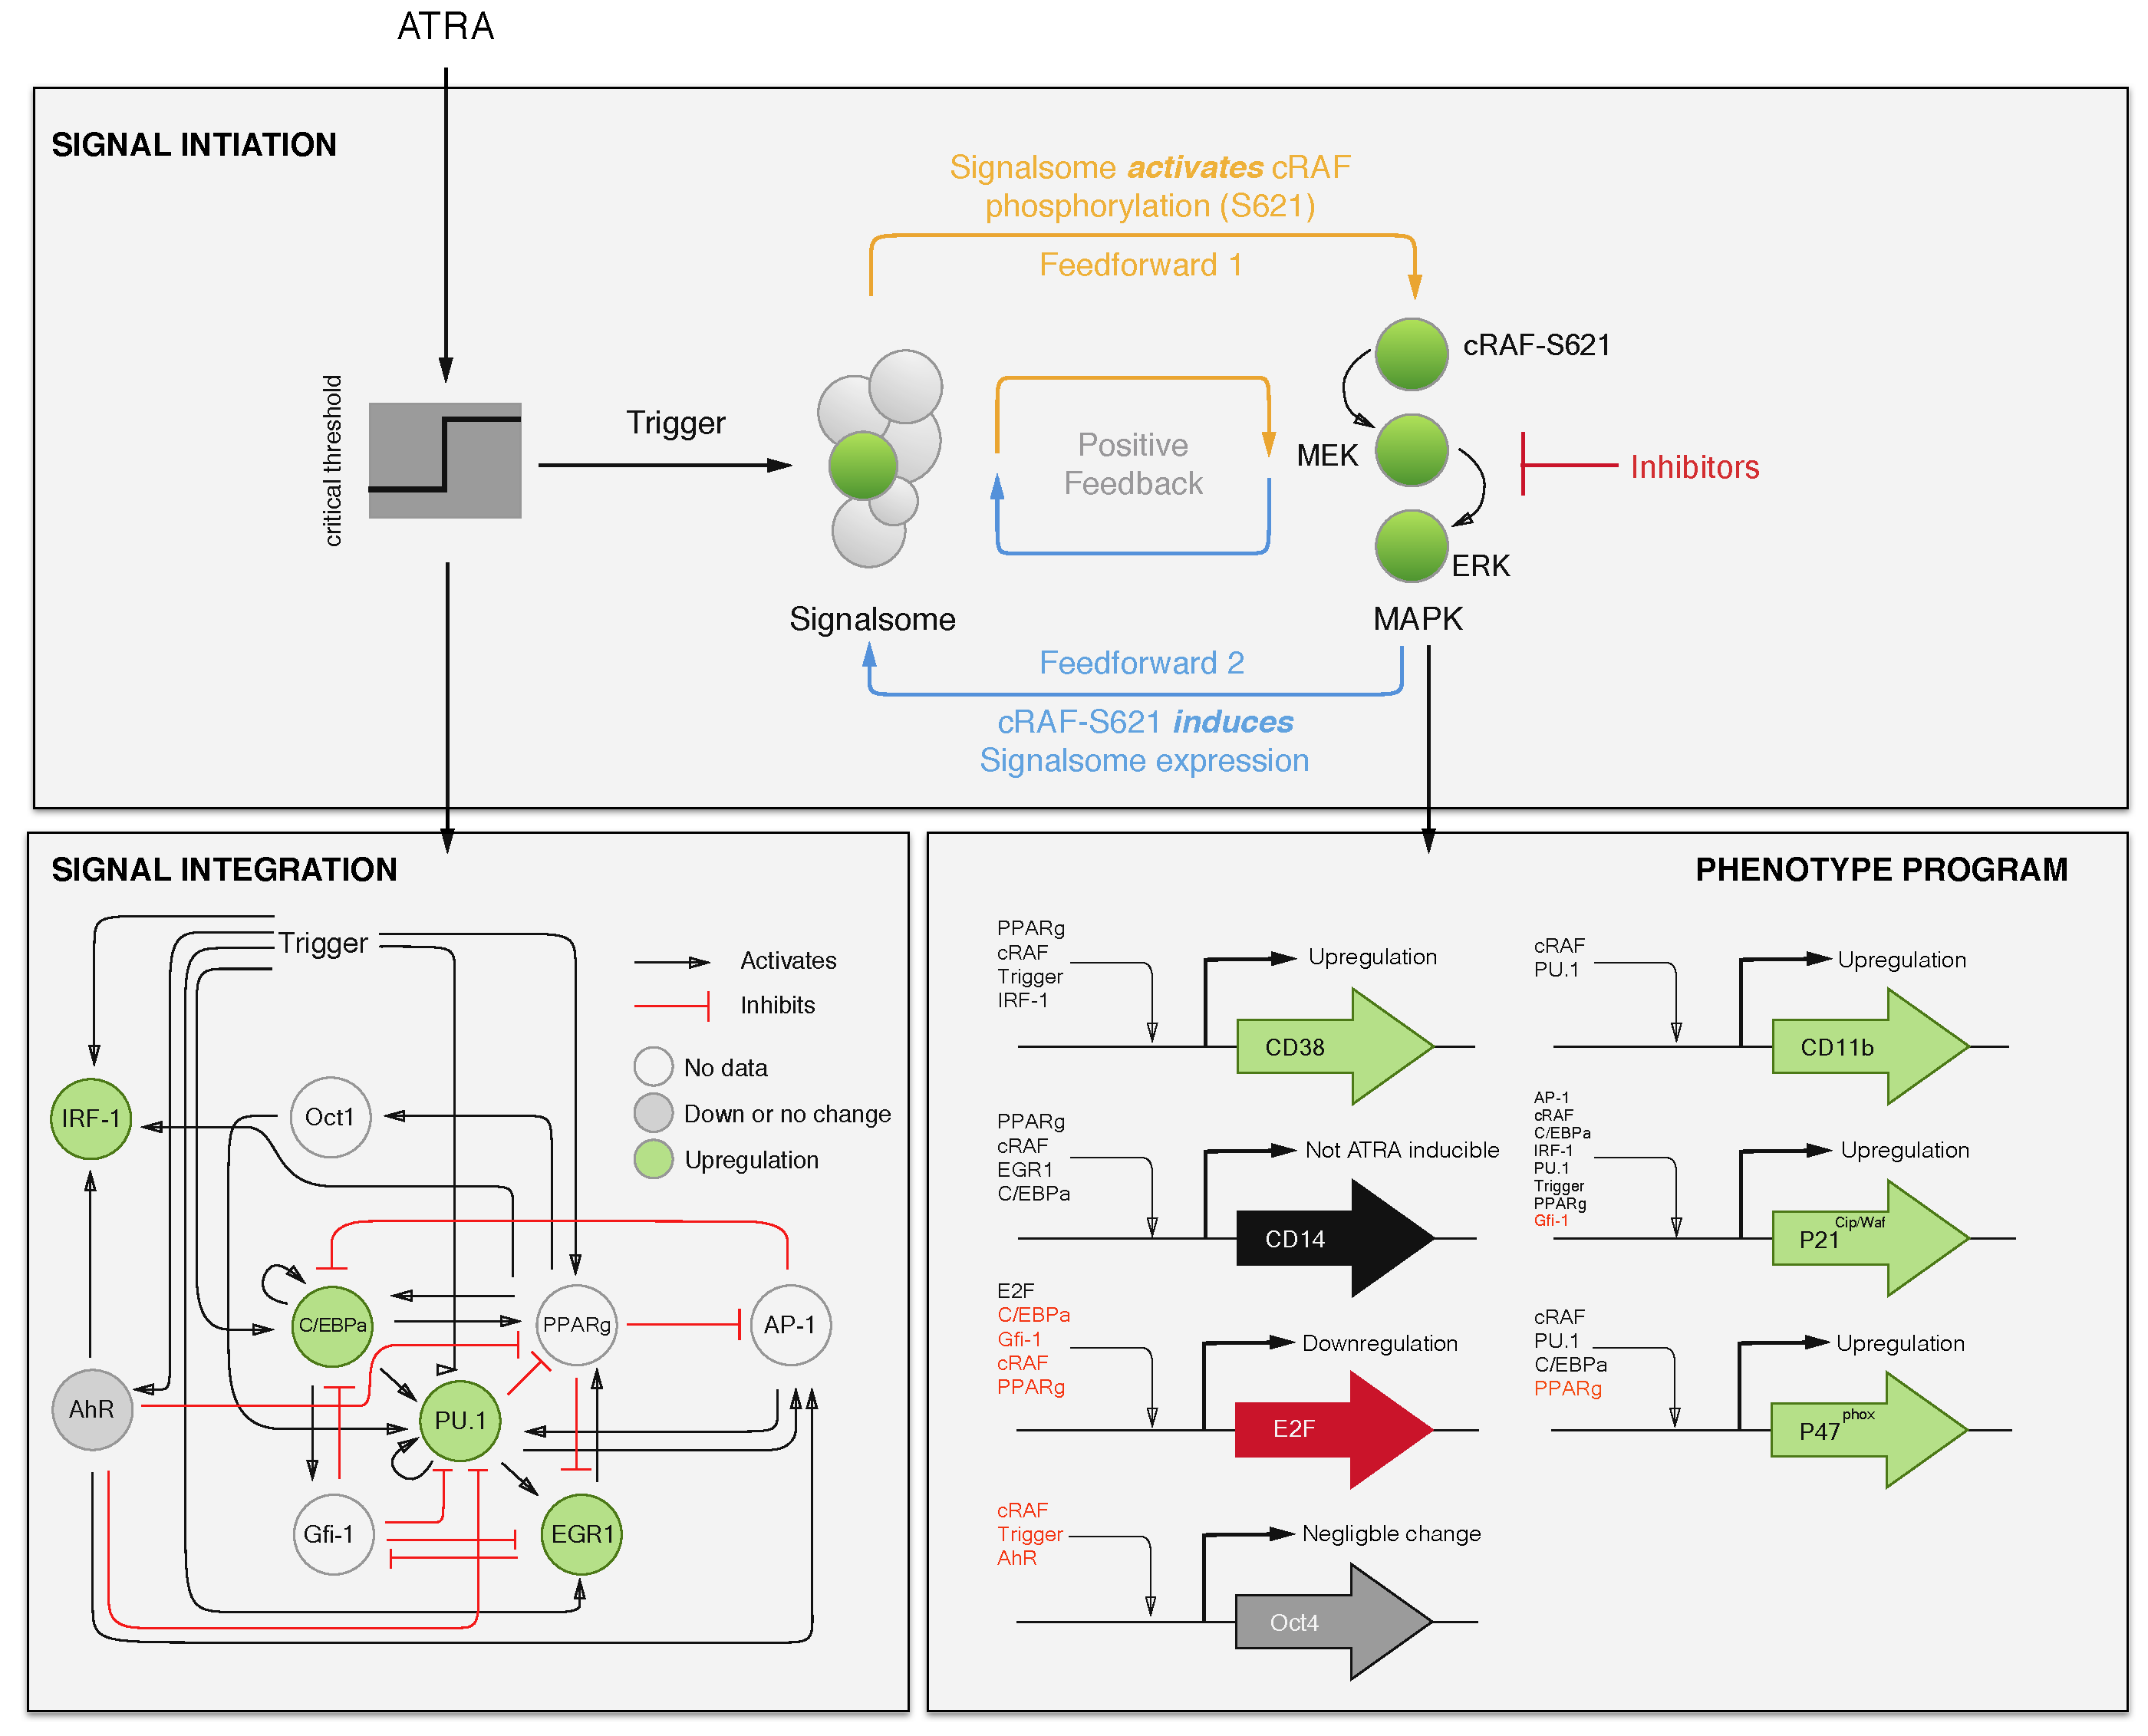
\includegraphics[width=1.0\textwidth]{./figs/Fig-1-Network_v3.pdf}
\caption{Schematic of the effective ATRA differentiation circuit.
Above a critical threshold, ATRA activates an upstream Trigger, which induces signalsome complex formation.
Signalsome activates the mitogen-activated protein kinase (MAPK) cascade which in turn
drives the differentiation program and signalsome formation.
Both Trigger and activated cRaf-pS621 drive a phenotype gene expression program responsible for differentiation.
Trigger activates the expression of a series of transcription factors which in combination with cRaf-pS621 result in phenotypic change.}\label{fig:network}
\end{figure}

\begin{figure}[!t]\centering
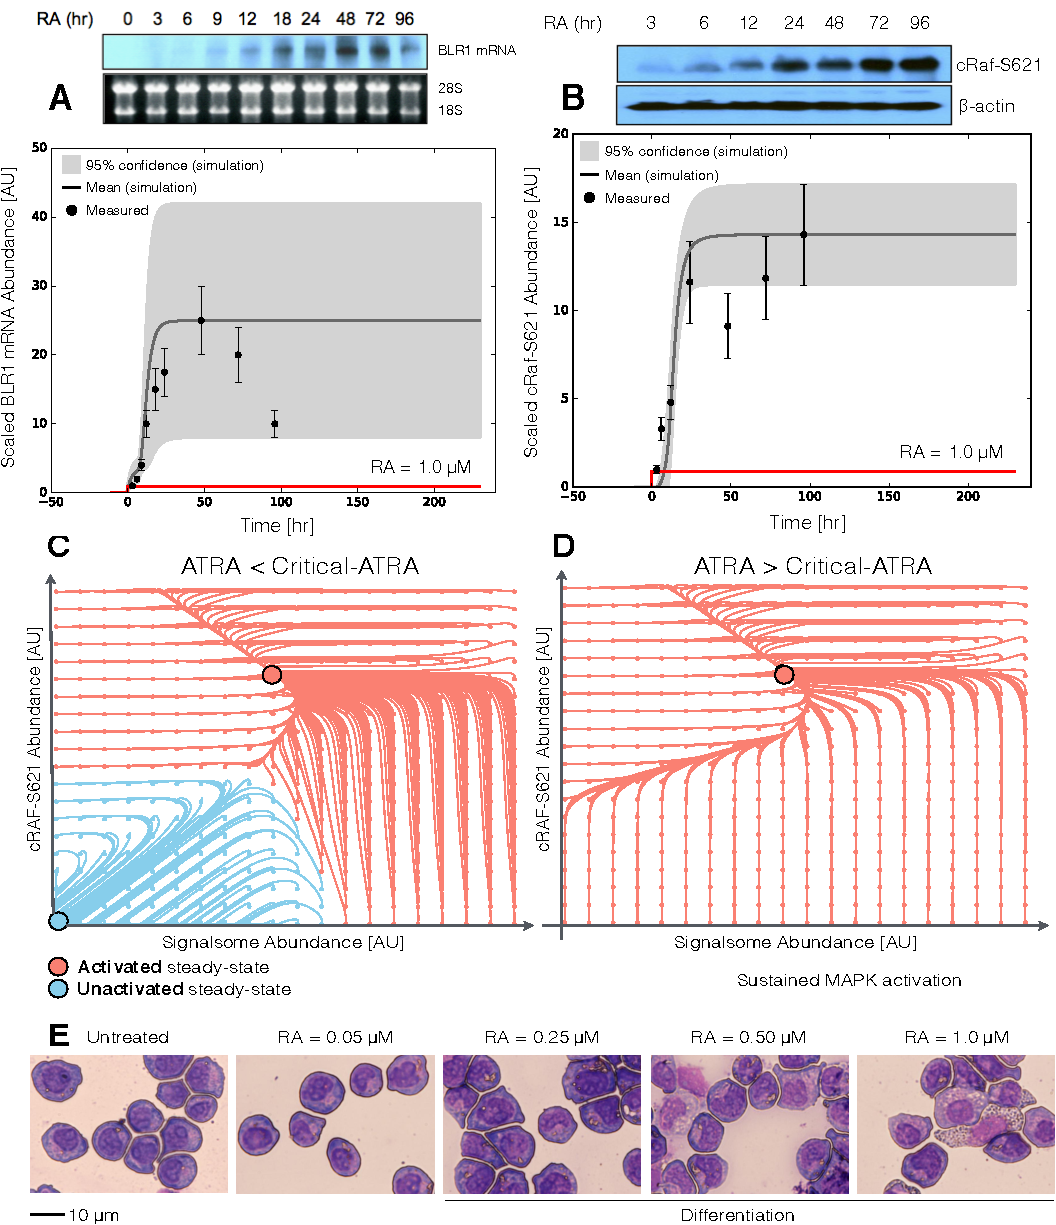
\includegraphics[width=0.90\textwidth]{./figs/Fig-2-cRaf-BLR1-Fit-Analysis.pdf}
\caption{Model analysis for ATRA-induced HL-60 differentiation.
A: BLR1 mRNA versus time following exposure to 1$\mu$M ATRA at t = 0 hr.
B: cRaf-pS621 versus time following exposure to 1$\mu$M ATRA at t = 0 hr.
Points denote experimental measurements, solid lines denote the mean model performance. Shaded regions denote the 99\% confidence interval calculated over the parameter ensemble.
C: Signalsome and cRaf-pS621 nullclines for ATRA below the critical threshold.
The model had two stable steady states and a single unstable state in this regime.
D: Signalsome and cRaf-pS621 nullclines for ATRA above the critical threshold.
In this regime the model had only a single stable steady state.
E: Morphology of HL-60 as a function of ATRA concentration (t = 72 hr). }\label{fig:model-fitting}
\end{figure}

\begin{figure}[!t]\centering
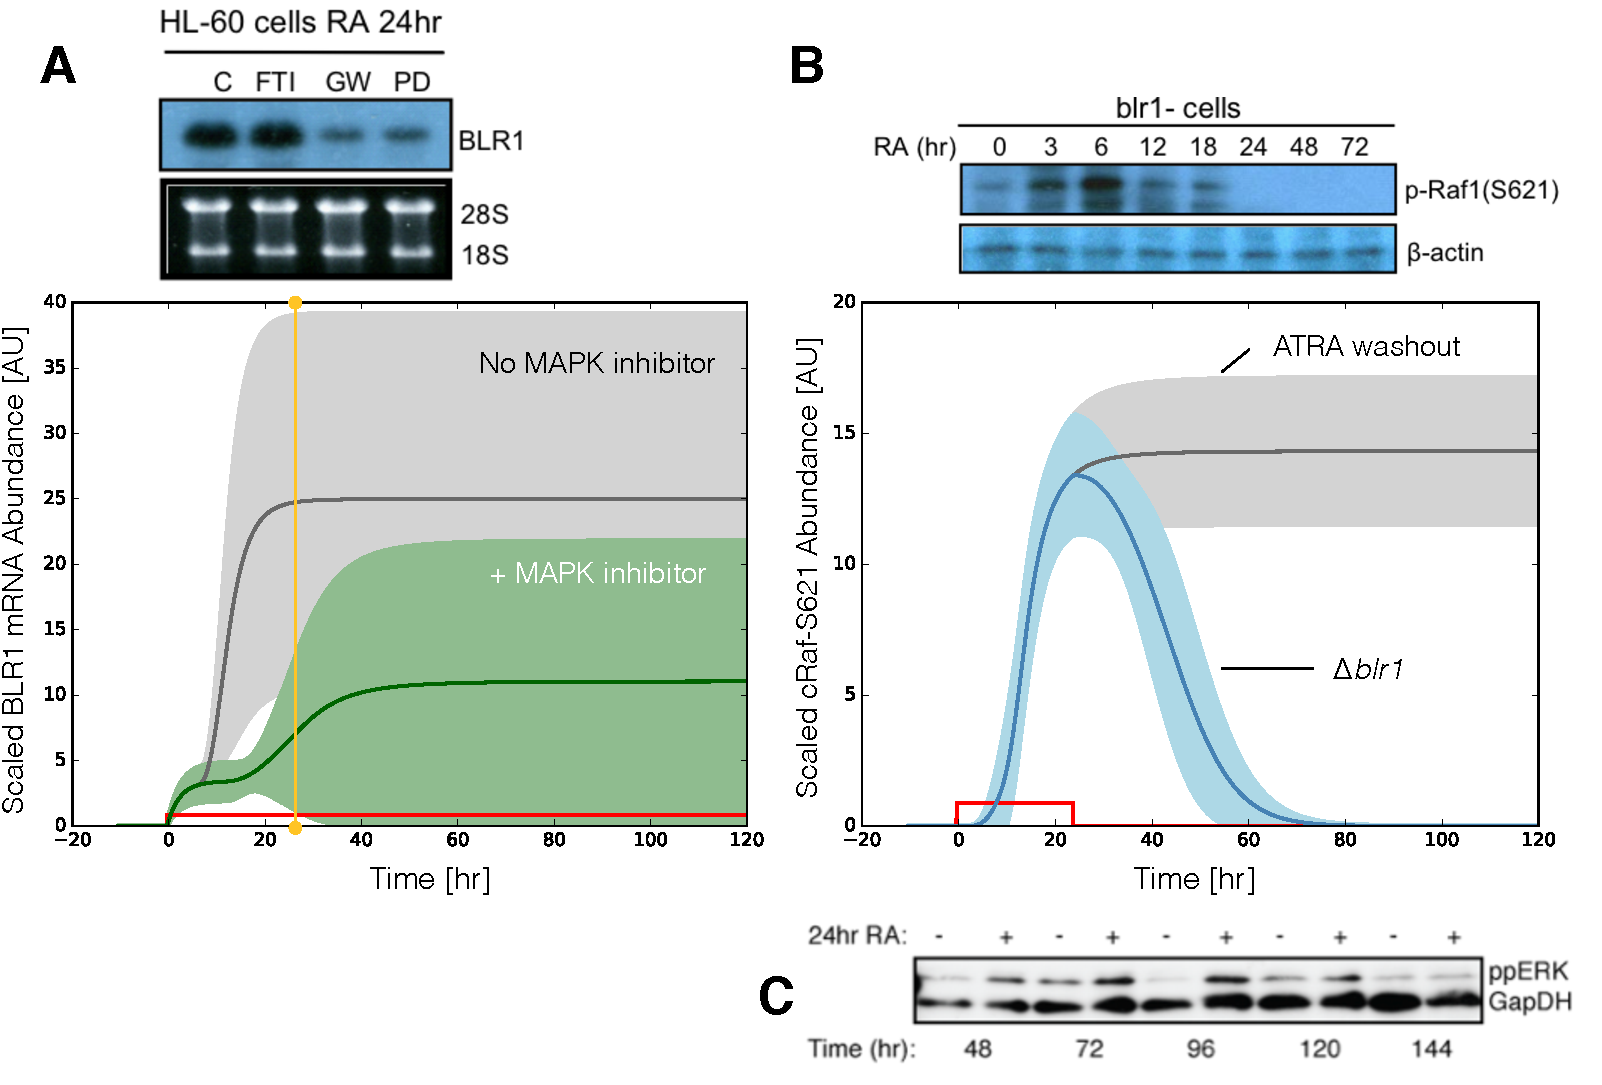
\includegraphics[width=1.0\textwidth]{./figs/Fig-3-Predictions.pdf}
\caption{Model simulation following exposure to 1$\mu$M ATRA.
A: BLR1 mRNA versus time with and without MAPK inhibitor.
B: cRaf-pS621 versus time following pulsed exposure to 1$\mu$M ATRA with and without BLR1.
Solid lines denote the mean model performance, while shaded regions denote the 99\% confidence interval calculated over the parameter ensemble.
C: Western blot analysis of phosphorylated ERK1/2 in ATRA washout experiments.
Experimental data in panels A and B were reproduced from Wang and Yen \cite{Wang2008}, data in panel C is reported in this study. }\label{fig:model-predictions}
\end{figure}

\begin{figure}[!t]\centering
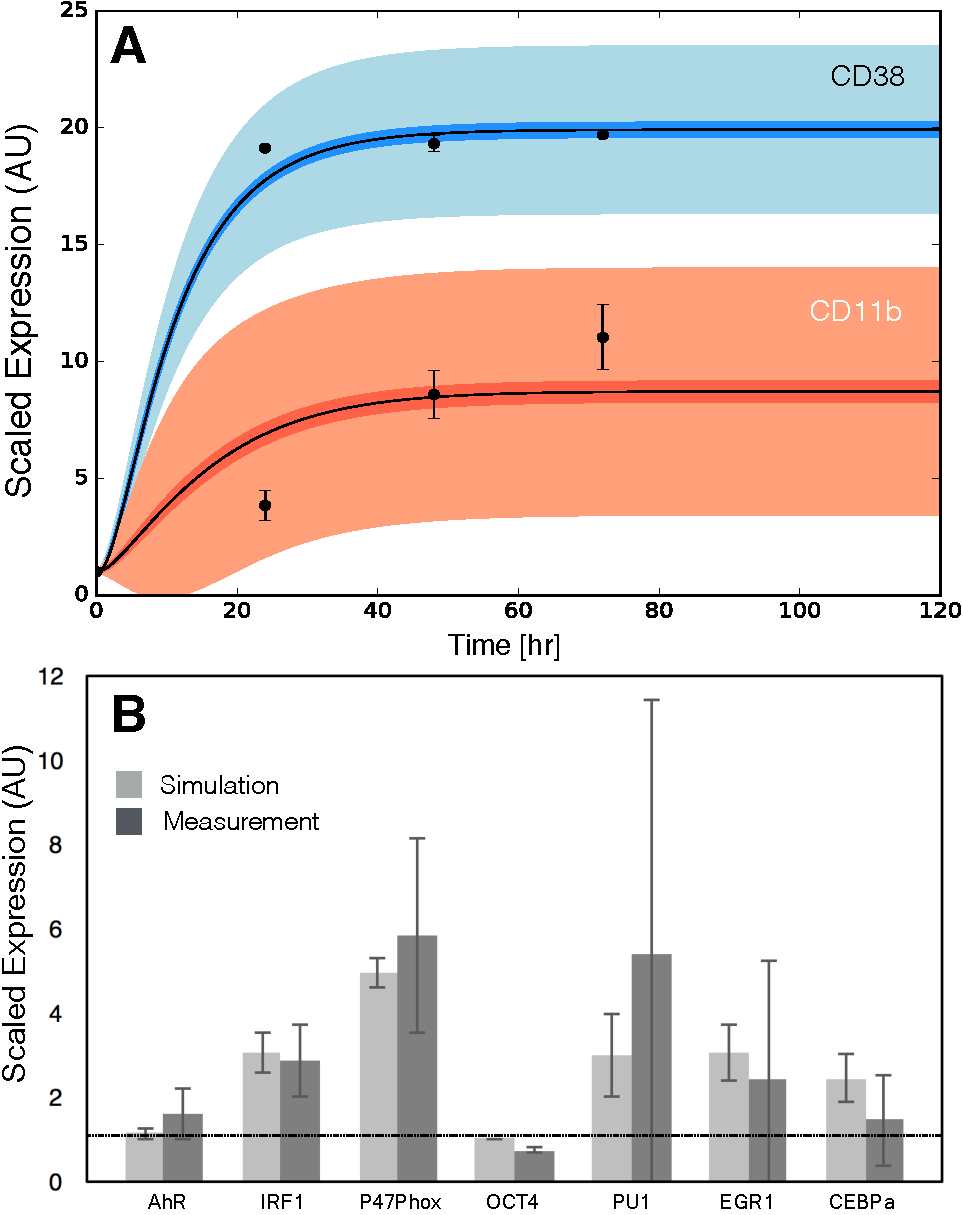
\includegraphics[width=0.85\textwidth]{./figs/Fig-5-GRN-Simulations.pdf}
\caption{Model simulation of the HL-60 gene expression program following exposure to 1$\mu$M ATRA at t = 0 hr.
A: CD38 and CD11b expression versus time following ATRA exposure at time t = 0 hr.
B: Gene expression at t = 48 hr following ATRA exposure.
Experimental data in panels A and B were reproduced from Jensen et al. \cite{Jensen:2015aa}.}\label{fig:model-grn-simulations}
\end{figure}

\begin{figure}[!t]
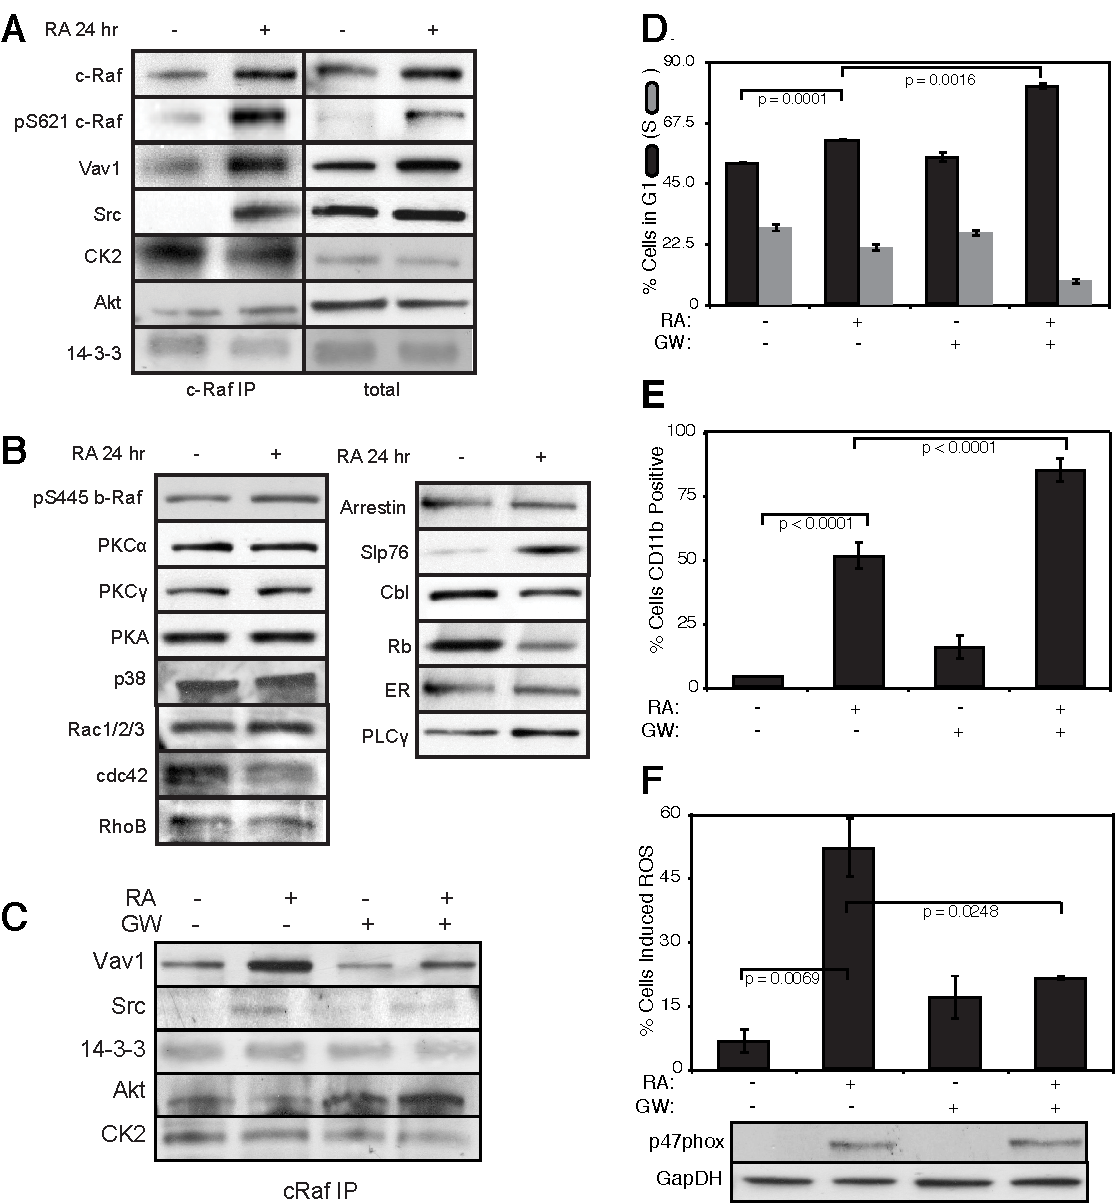
\includegraphics[width=0.9\textwidth]{./figs/Fig-1-IP-ExperimentalStudies.pdf}
\caption{Investigation of a panel of possible Raf interaction partners in the presence and absence of ATRA.
A: Species identified to precipitate out with Raf:
first column shows Western blot analysis on total Raf immunoprecipitation with and without 24 hr ATRA treatment
and the second on total lysate.
B: The expression of species considered that did not precipitate out with Raf at levels detectable by Western blot analysis on total lysate.
C: Effect of the Raf inhibitor GW5074 on Raf interactions as determined by Western blot analysis of total Raf immunoprecipitation.
The Authors note the the signal associated with Src was found to be weak.
D: Cell Cycle distribution as determined by flow cytometry indicated arrest induced by ATRA, which was increased by the addition of GW5074.
E: Expression of the cell surface marker CD11b as determined by flow cytometry indicated increased expression induced by ATRA,
which was enhanced by the addition of GW5074.
F: Inducible reactive oxygen species (ROS) as determined by DCF flow cytometry. The functional differentiation response of ATRA treated cells
was mitigated by GW5074.}\label{fig:ip-data}
\end{figure}

\clearpage

% Supplemental figures -
% Set the S-
\renewcommand\thefigure{S\arabic{figure}}
\renewcommand\thetable{T\arabic{table}}
\renewcommand\thepage{S-\arabic{page}}
\renewcommand\theequation{S\arabic{equation}}

% Reset the counters -
\setcounter{equation}{0}
\setcounter{table}{0}
\setcounter{figure}{0}
\setcounter{page}{1}


\end{document}
